% ==========================================================================
\section{Appendixes}
% ==========================================================================
\label{sec:appendixes}

    % ==========================================================================
    \subsection{ANSI Terminal colours}
    % ==========================================================================

    \begin{itemize}
        \item ANSI\_COLR\_BLK - Black
        \item ANSI\_COLR\_RED - Red
        \item ANSI\_COLR\_GRN - Green
        \item ANSI\_COLR\_YLW - Yellow
        \item ANSI\_COLR\_BLU - Blue
        \item ANSI\_COLR\_MGT - Magenta
        \item ANSI\_COLR\_CYA - Cyan
        \item ANSI\_COLR\_WHT - White
    \end{itemize}

    % ==========================================================================
    \subsection{VDP Composite colours}
    % ==========================================================================
    \label{sec:vdp_colours}

    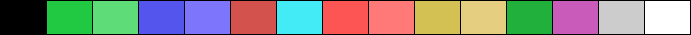
\includegraphics[scale=0.7]{images/TMS9918Apalette.png}

    \begin{itemize}
        \item VDP\_COLR\_TRNSP  (Transparent)   = \$00
        \item VDP\_COLR\_BLACK  (Black)         = \$01
        \item VDP\_COLR\_M\_GRN (Medium Green)  = \$02
        \item VDP\_COLR\_L\_GRN (Light Green)   = \$03
        \item VDP\_COLR\_D\_BLU (Dark Blue)     = \$04
        \item VDP\_COLR\_L\_BLU (Light Blue)    = \$05
        \item VDP\_COLR\_D\_RED (Dark Red)      = \$06
        \item VDP\_COLR\_CYAN   (Cyan)          = \$07
        \item VDP\_COLR\_M\_RED (Medium Red)    = \$08
        \item VDP\_COLR\_L\_RED (Light Red)     = \$09
        \item VDP\_COLR\_D\_YLW (Dark Yellow)   = \$0A
        \item VDP\_COLR\_L\_YLW (Light Yellow)  = \$0B
        \item VDP\_COLR\_D\_GRN (Dark Green)    = \$0C
        \item VDP\_COLR\_MGNTA  (Magenta)       = \$0D
        \item VDP\_COLR\_GREY   (Grey)          = \$0E
        \item VDP\_COLR\_WHITE  (White)         = \$0F
    \end{itemize}

    % ==========================================================================
    \subsection{VDP Screen resolutions}
    % ==========================================================================
    \label{sec:vdpscrmodes}


        % ==========================================================================
        \subsubsection{Mode 0: \textbf{Text Mode}}
        % ==========================================================================
        \begin{itemize}
            \item Screen is divided into 960 pattern positions each of which is
                capable of displaying a character. There are 40 characters in
                each row and 24 rows on the screen.
            \item Each character is 8x6 pixels.
            \item Each character can have 2 colours (Foreground and Background).
            \item Sprites cannot be used.
            \item The Pattern Table starts at \textbf{VRAM} address
                \texttt{0x0000}, for a lenght of 2048 bytes (from
                \texttt{0x0000} to \texttt{0x07FFF}).
            \begin{itemize}
                \item This table contains the character sets, for a maximum of
                    256 characters per set.
                \item Up to 7 different character sets can be held in the
                    \textbf{VRAM} at the same time. Each set MUST be located
                    starting at an \texttt{0x0800} boundary (i.e. 
                    \texttt{0x0000}, \texttt{0x1000}, \texttt{0x1800},
                    \texttt{0x2000}, \texttt{0x2800}, \texttt{0x3000} and
                    \texttt{0x3800}). Note that \texttt{0x0800} is not listed
                    because that address is used by the Name Table.
                \item Ideally, the patterns follow the ASCII table definitions
                    and order, so that the Name Table can be easily used to
                    display text by for example assigning the value \texttt{0x41}
                    to a byte in the Name Table to display the character
                    \textit{A}.
            \end{itemize}
            \item The Name Table starts at \textbf{VRAM} address \texttt{0x0800}.
                for a lenght of 960 bytes (from \texttt{0x0800} to
                \texttt{0x0BBF}).
            \begin{itemize}
                \item Each entry in the table is 1 byte long and therefore can
                    specify one of 256 patterns (from \texttt{0x00} to
                    \texttt{0xFF}).
                \item Each entry represents a pattern position on the screen.
                    Position 0 is in the top left of the screen. Position 39 is
                    in the top right of the screen. The second row ranges from
                    40 to 79, and so on.
            \end{itemize}
        \end{itemize}

        % ==========================================================================
        \subsubsection{Mode 1: \textbf{Graphics I Mode}}
        % ==========================================================================
        \begin{itemize}
            \item Screen is divided into 768 blocks of 8x8 pixels each. There
                are 32 blocks in a row and 24 rows on the screen.
            \item Sprites can be used.
            \item The Name Table starts at \textbf{VRAM} address \texttt{0x1400}.
            \begin{itemize}
                \item This table has 768 entries, one for each block on the screen.
                \item If the Pattern Table is loaded with with a full ASCII
                    character set, the entry of any ASCII value in the Name
                    Table will result in the corresponding character being
                    displayed on the screen.
            \end{itemize}
            \item The Pattern Table starts at \textbf{VRAM} address \texttt{0x0800}.
            \item The Colour Table starts at \textbf{VRAM} address \texttt{0x2000}.
            \begin{itemize}
                \item This table has 32 entries, each entry defining 2 colours
                (Foreground and Background) out of 15 colours available, for a
                block of 8 characters. In other words, colours cannot be
                assigned independently to each character in the screen, but
                instead to groups of 8 consecutive characters.
            \end{itemize}
        \end{itemize}

        % ==========================================================================
        \subsubsection{Mode 2: \textbf{Graphics II Mode}}
        % ==========================================================================
        \begin{itemize}
            \item Also known as \textbf{Bitmap Mode}.
            \item Screen is divided into 768 blocks of 8x8 pixels each. There
            are 32 blocks in a row and 24 rows on the screen.
            \item Sprites can be used.
            % \item Screen resolution is 256 by 192 pixels.
            \item The Name Table starts at \textbf{VRAM} address \texttt{0x3800}.
            \begin{itemize}
                \item This table is divided into three subtables of 256 each.
            \end{itemize}
            \item The Pattern Table starts at \textbf{VRAM} address \texttt{0x0000}.
            \item The Colour Table starts at \textbf{VRAM} address \texttt{0x2000}.
            \begin{itemize}
                \item Each entry in the Colour Table is 8 bytes and each byte
                    defines the 2 colours (Foreground and Background) of each 
                    of the 8 rows of the character, from a total of 15 colours
                    plus transparent available.
            \end{itemize}
        \end{itemize}

        % ==========================================================================
        \subsubsection{Mode 3: \textbf{Multicolour Mode}}
        % ==========================================================================
        \begin{itemize}
            \item Screen is divided into 768 blocks of 2x2 squares. Each square
                is 4 pixels. There are 32 blocks in each row and 4 rows in each
                section. There are 6 sections, for a total of 24 rows on the
                screen.
            \item Blocks are arranged in columns with 4 blocks in each column.
            \item Columns are arranged in sections, with 32 columns in each
                section.
            \item There are a total of 6 sections on the screen.
            \item In summary:
            \begin{itemize}
                \item 32 columns * 6 sections = 192 columns
                \item 192 columns * 4 blocks = 768 blocks
            \end{itemize}
            \item No characters for text can be used.
            \item Sprites can be used.
            \item The Name Table starts at \textbf{VRAM} address \texttt{0x1400}.
            \item The Colour Table is not used. Instead, the colour of the boxes
            are defined in the Pattern Table.
            \item The Pattern Table starts at \textbf{VRAM} address \texttt{0x0800}.
            \begin{itemize}
                \item Each entry in the table is 8 bytes, but only 2 bytes are
                        used to define the colours of the 4 boxes that make up
                        a character.
            \end{itemize}
        \end{itemize}

        % ==========================================================================
        \subsubsection{Mode 4: \textbf{Graphics II Mode Bitmapped}}
        % ==========================================================================
        \begin{itemize}
            \item Same as Mode 2, but screen is bitmapped for addressing every
                pixel individually.
        \end{itemize}

    % ==========================================================================
    \subsection{VDP Limitations}
    % ==========================================================================

    The maximum resolutions are: 240x192 pixels in Text Mode, 256x192 pixels in
    Graphics Modes (I, II, II Bit-mapped), and 512x384 in Multicolour Mode.

    The maximum number of colours is 15 plus a transparent colour.

    In Graphics I Mode, each entry in the Colour Table defines the colour for
    a group of eight patterns. Hence, individual character colouring is not
    possible.

    In Graphics II Bit-mapped Mode, individual pixels can be addressed but
    individual colours cannot. Therefore it is not possible to assign different
    colours for each pixel.

    % ==========================================================================
    \subsubsection{Sprites}
    % ==========================================================================

    A maximum of 32 sprites can be shown on the screen, of sizes either 8x8 or
    16x16 pixels. Though sprites can be magnified, thus showing as 16x16 or
    32x32 respectively.

    The location of a sprite is defined by the top left-hand corner of the
    sprite pattern.

    When more than one sprite is located at the same screen coordinate, the
    sprite on the higher priority plane will be shown.

    A maximum of 4 sprites can be displayed on the same horizontal line. If this
    rule is violated, the four highest priority sprites on the line are
    displayed normally, but the fifth and subsequent sprites are not displayed.

    The \textit{Coincidence Flag} (collision dectection) only indicates that
    any two sprites have overlapping bits, but it does not tell which sprites
    are. This must be calculated programatically.

    % ==========================================================================
    \subsection{Jiffy Counter}
    % ==========================================================================
    \label{subsec:jiffy_counter}

    A \textit{Jiffy} is the time between two ticks of the system timer interrupt.
    On the dastaZ80, this timer is generated by the TMS9918A (\textbf{VDP}) at
    roughly each 1/60th second.\\

    The counter is made of 3 bytes. Byte 1 is incremented in each \textbf{VDP}
    interrupt. Once it rolls over to zero (256 increments), the byte 2 is
    incremented. Once the byte 2 rolls over, the byte 3 is incremented. Once the
    three bytes together (24-bit) reach the value \texttt{0x4F1A00}, the three
    bytes are initialised to zero.

    \texttt{0x4F1A00} (5,184,000 in decimal) is the number of jiffies in 24
    hours: 24 hours x 60 minutes in an hour x 60 seconds in a minute x 60
    jiffies in a second.

    \textbf{IMPORTANT}: This counter MUST not be interpreted as an accurate
    clock, because when transferring data to the \textbf{VRAM} the OS disables
    the \hyperref[sec:nmi]{NMI}\footnote{It is also highly recommended that in
    your programs you also disable the \hyperref[sec:nmi]{NMI} when copying
    large amounts of data. Otherwise, the process will be interrupted 60 times
    per second, and therefore slow it down.}, and therefore the counter stops
    for a while.

    % ==========================================================================
    \subsection{OS Boot Sequence}
    % ==========================================================================
    After power on or after pressing the \textbf{RESET} button:

    \begin{itemize}
        \item \textbf{Bootstrap}
        \begin{itemize}
            \item Copy contents of the ROM into High RAM (\texttt{0x8000} - \texttt{0xFFFF}).
            \item Disable ROM chip and enable Low RAM (\texttt{0x0000} - \texttt{0x7FFF}).
            Therefore, all \textbf{MEMORY} is RAM from now on.
            \item Copy the copy of ROM inm High RAM to Low RAM. Bootstrap code is not copied.
            \item Transfer control to BIOS (\texttt{jp F\_BIOS\_SERIAL\_INIT}).
        \end{itemize}
        \item \textbf{Initialise SIO/2} (\texttt{F\_BIOS\_SERIAL\_INIT})
        \begin{itemize}
            \item Initialise SIO/2.
            \begin{itemize}
                \item Set Channel A as 115,000 bps, 8N1, Interrupt in all 
                received characters.
                \item Set Channel B as 115,000 bps, 8N1, Interrupt in all 
                received characters.
                \item Set Interrupt Vector to \texttt{0x60}.
            \end{itemize}
            \item Set CPU to Interrupt Mode 2.
            \item \texttt{jp F\_BIOS\_WBOOT}
        \end{itemize}
        \item \textbf{BIOS Boot} (\texttt{F\_BIOS\_WBOOT})
        \begin{itemize}
            \item Set SIO/2 Channel A as primary I/O.
            \item Transfer control to Kernel (\texttt{jp F\_KRN\_START}).
        \end{itemize}
        \item \textbf{Kernel Boot} (\texttt{F\_KRN\_START})
        \begin{itemize}
            \item Display dzOS welcome message.
            \item Display dzOS release version.
            \item Display Kernel version.
            \item Display available \textbf{RAM}.
            \item Initialise \textbf{VDP}.
            \begin{itemize}
                \item Test write/read \textbf{VRAM}.
                \item Set \textbf{Low Resolution Display} as \textit{Graphics II
                Bit-mapped Mode}.
                \item Show dastaZ80 Logo in the \textbf{Low Resolution Display}.
            \end{itemize}
            \item Initialise \textbf{PSG}.
            \begin{itemize}
                \item Set Noise OFF, Audio OFF, I/O Port as Output.
                \item Make a beep.
            \end{itemize}
            \item Initialise \textbf{FDD}.
            \item Initialise \textbf{SD Card}.
            \begin{itemize}
                \item Detect \textbf{SD Card}.
                \item Display number of available Disk Image Files.
                \item Display disk unit and name of each Disk Image File.
            \end{itemize}
            \item Initialise \textbf{Real-Time Clock (RTC)}.
            \begin{itemize}
                \item Detect \textbf{RTC}.
                \item Display current date and time.
                \item Display \textbf{RTC}'s battery status.
                \item Detect \textbf{NVRAM}.
            \end{itemize}
            \item Initialise \hyperref[sec:ram_memmap]{SYSVARS}.
            \begin{itemize}
                \item Set show deleted files with \textit{cat} command as OFF.
                \item Set default File Type as 0 (USR = User defined).
                \item Set default loadsave address to \texttt{0x0000} (i.e. will
                save/load starting from \hyperref[subsec:memmap:ram]{Free RAM}
                (\texttt{0x4420})).
            \end{itemize}
            \item Set default \textbf{DISK} as 1 (i.e. first Disk Image File in
            the \textbf{SD card}).
            \item Transfer control to Command-line Interpreter (CLI) (\texttt{jp F\_CLI\_START}).
        \end{itemize}
        \item \textbf{CLI} (\texttt{F\_CLI\_START})
        \begin{itemize}
            \item Display CLI version.
            \item Clear command buffers
            \item Display prompt ($>$).
            \item Read command entered by user.
            \item Parse command.
            \item Execute corresponding subroutine.
            \item Loop back to Display prompt.
        \end{itemize}
    \end{itemize}

    % ==========================================================================
    \subsection{dzOS Programming Style}
    % ==========================================================================

    When writting dzOS and software for dzOS, the following style has been
    followed:

    \begin{itemize}
        \item All CPU registers are witten in uppercase (e.g. \textit{A},
        \textit{BC}, \textit{HL}, \textit{IX}, \textit{SP}).
        \item All CPU flags are witten in lowercase (e.g. \textit{z},
        \textit{nz}, \textit{c}, \textit{nc}, \textit{m}, \textit{p}).
        \item All assembly mnemonics are written in lowercase (e.g. 
        \textit{ld A,0}).
        \item Labels for subroutines that will be public (i.e. called via a
        Jumpblock) are written in uppercase.
        \item Labels are written in a line, with no mnemonics.
        \item Public subroutines contain comments specifying:
        \begin{itemize}
            \item Short description.
            \item Input CPU registers or variables (\hyperref[sec:ram_memmap]{SYSVARS}).
            \item Output CPU registers or variables (\hyperref[sec:ram_memmap]{SYSVARS}).
        \end{itemize}
        \item All hexadecimal values are written with a dollar sign as prefix.
        \item Tabulation (Tabs) are written as 4 spaces.
        \item Mnemonics start after 2 tabs (8 spaces).
        \item When possible, comments are written in column 41. Otherwise in
        next closest Tab.
        \item Source code is heavily commented. Mostly on each line.
        \item \textit{The Telemark Assembler} (TASM) specific:
        \begin{itemize}
            \item \textit{.BYTE} is used instead of \textit{.DB}
            \item \textit{.WORD} is used instead of \textit{.DW}
        \end{itemize}
    \end{itemize}